\section{Scattering from Clusters of Particles}
\label{sec:ours_theory}
%
%\sz{We should add a table of symbols with ``links'' to their definitions.}
%
In this section, we present our main theoretical result: the far-field approximated scattering dyad relating a field incoming at a particle, which will be shown in \Eq{eq:farscatdyad}.
This dyad can then be used to compute a medium's bulk scattering parameters, which we will discuss in \S\ref{ssec:ours_RTT}.

The two forms of computing the exciting field from particle $j$ to $i$ [\Eqs{eq:excfield}{eq:excfieldfar}] suggest that we can consider two subsets of particles $j$ depending on their distance with respect to the point of interest $\px$: One set of $\Nnear$ particles in the near field and another set of $\Nfar$ particles in the far field. With that, we can now calculate the exciting field in particle $i$ as:
%
\begin{equation}
    \EField_i(\px)= \IncEField(\px) + \sum_{j(\neq i)=1}^\Nnear \ExcEField_{ij}(\px) + \sum_{k=1}^\Nfar \ExcEField_{ik}(\px).
    \label{eq:foldylaxtwo}
\end{equation}

In what follows, we derive the far-field Foldy-Lax equations for groups of particles where a cluster of these particles are in their respective near-field region, while the other elements in the system are in the far field. For the simplicity of our derivations, we consider a single far-field incident field in the cluster, and assume that the far-field particles $k$ do not have neighbor particles in their respective near field region.
%
More formally, we now consider a cluster $\Cls$ of $N_\Cls$ particles, where all particles $i\in\Cls$ are in their respective near-field region, and that the particles of the cluster have a bounding sphere centered at $\Px_\Cls$ with radius $\radius_\Cls$ (see Figure~\ref{fig:diagram}, middle). 

Since both the incident field $\IncEField(\px)$ and the exciting field $\ExcEField_{\Cls k}(\px)$ from particle $k$ are in the far-field region, we can assume both fields to be planar waves defined as
%
\begin{align}
    \label{eq:farincfieldcluster}
    \IncEField(\px) &= \IncEField_0 \,\exp(\img k_1 \dw \cdot \Delta \px) = \IncEField_0\,\sGreenProp(\dw, \Delta \px) , \\
    \ExcEField_{\Cls k}(\px) &= \ExcEField_{0\Cls k}\,\exp(\img k_1 \dPx_{\Cls k} \cdot \Delta \px) =  \ExcEField_{0\Cls k}\,\sGreenProp(\dPx_{\Cls k}, \Delta \px), 
    \label{eq:farexcfieldcluster} 
\end{align}
%  
with $\IncEField_0$ the amplitude of the planar incident field, $\dw$ its direction, and $\Delta \px=\px-\Px_\Cls$. Equivalently, $\ExcEField_{0\Cls k}=\frac{\exp(\img k_1 \,\tPx_{\Cls k})}{\tPx_{\Cls k}}\,\ExcEField_{1\Cls k}(\dPx_{\Cls k})$  is the amplitude of the exciting field at $\Cls$ from particle $k$, and $\dPx_{\Cls k}$ its direction. 

Now, let us slightly abuse the dot product notation, remove the dependency on the spatial dependency on each term, and use $(\varphi_1 \cdot \varphi_2) = \int \varphi_1(x)\,\varphi_2(x) \diff x$ for scalar-valued functions $\varphi_1$ and $\varphi_2$. From the far-field assumptions, plugging \Eq{eq:foldylaxtwo} into the definition of the scattered field from particle $i\in\Cls$ in Equation~\eqref{eq:foldylax} (with $\Nnear=\Ncls$) yields
%
\begin{equation}
    \label{eq:scafieldcluster1}
    \begin{split}
        \ScaEField_i(\px) &= \sGreen \cdot \dyad{T}_i\cdot \EField_i\\
        & = \sGreen \cdot \dyad{T}_i \cdot \left[\IncEField + \sum_{k=1}^\Nfar \ExcEField_{\Cls k}+ \sum_{j(\neq i)=1}^\Ncls \ExcEField_{ij} \right].
    \end{split}        
\end{equation}
%
By recursively expanding $\ExcEField_{ij}$ and some algebraic operations (see the supplemental for the full derivation), this results into 
\begin{align}
    \label{eq:scafieldcluster5}
    \ScaEField_i(\px) &= \EField_0 \, \sGreen \cdot \dyad{T}_i \cdot \Bigg[ \sGreenProp(\dw) + \sum_{j(\neq i)=1}^\Ncls \left[...\right]_j^{\sGreenProp(\dw)} \Bigg] \\
    & + \sum_{k=1}^\Nfar \ExcEField_{0\Cls j}\,\left[ \sGreen \cdot \dyad{T}_i \cdot \Bigg[ \sGreenProp(\dPx_{\Cls k}) + \sum_{j(\neq i)=1}^\Ncls \left[...\right]_j^{\sGreenProp(\dPx_{\Cls k})}\Bigg]\right]. \nonumber 
\end{align}
%
where the "$[...]_l^\varphi$" term represents the recursivity as
%
\begin{equation}
    [...]_j^\varphi= \sGreen \cdot \dyad{T}_j \cdot \left[\varphi + \sum_{l(\neq j)=1}^\Ncls \left[...\right]_l^\varphi\right] \,.
\end{equation}
%
Note that each element in the sum in \Eq{eq:scafieldcluster5} above is the result of the amplitude of the far-field incident or exciting fields, and a series that encode all the near-field scattering in the cluster $\Cls$. We can thus define the scattering dyad $\ScaDyad_i^\text{near}(\dwi,\px)$ relating a unit-amplitude planar incident field at particle $i$ from direction $\dwi$ with the scattered field at point $\px$ as
%
\begin{equation}
    \ScaDyad_i^\text{near}(\dwi,\px) = \sGreen \cdot \dyad{T}_i\cdot \Bigg[ \sGreenProp(\dwi) + \sum_{j(\neq i)=1}^\Ncls \left[...\right]_j^{\sGreenProp(\dwi)} \Bigg].
    \label{eq:scatdyad_near}
\end{equation}
%
By considering constant $\IncEField_0$ and $\ExcEField_{0\Cls k}$ for the whole cluster $\Cls$, we can compute the cluster's scattering dyad as:
%
\begin{equation}
    \ScaDyad_\Cls^\text{near}(\dwi,\px) = \sum_{i=1}^{N_\Cls} \ScaDyad_i(\dwi,\px),
    \label{eq:scatdyadcluster_near}
\end{equation}
%
%The scattering dyad $\ScaDyad_\Cls^\text{near}(\dwi,\px)$ solves
which defines the scattered field for a unit-amplitude incoming planar field in a scene consisting of the particles forming cluster $\Cls$.
In practice, the scattering dyad $\ScaDyad_\Cls^\text{near}(\dwi,\px)$ can be computed numerically using standard methods from computational electromagnetics~\cite{mishchenko2014electromagnetic}.


\paragraph{Far-field approximation}
\Eq{eq:scatdyad_near} represents the general form of the scattering dyad for particle $i$, which results into a five-dimensional function. Assuming that $\px$ is in the far-field region of a particle $i\in\Cls$, by using the far-field approximation of the scattered or exciting field~\eqref{eq:excfieldfar} (we refer to the supplemental document for the derivation), we get the scattered field by particle $i$ as
%
\begin{align}
    \ScaEField_i(\px) \approx \frac{\E^{\img k_1 \tPx_i}}{\tPx_i} \Big(\EField_0 \,  \ScaDyad_i(\dw,\dPx_i) 
    + \sum_{k=1}^\Nfar \ExcEField_{0\Cls k} \, \ScaDyad_i(\dPx_{\Cls k},\dPx_i) \Big),
    \label{eq:farscatfield}
\end{align}
%
with $\tPx_i=|\px-\Px_i|$ and $\dPx_i=\frac{\px-\Px_i}{\tPx_i}$, and %$\ScaDyad_i(\dwi,\dws)$ the scattering dyad relating incident and scattered directions $\dwi$ and $\dws$ as
\begin{equation}
    \label{eq:farscatdyad}
    \boxed{%
        \ScaDyad_i(\dwi,\dws) = \frac{g(\dws)\cdot \dyad{T}_i}{4\pi} \cdot\Bigg[ \sGreenProp(\dwi) + \sum_{j(\neq i)=1}^\Ncls \left[...\right]_j^{\sGreenProp(\dwi)} \Bigg].
    }
\end{equation}
%
Finally, since $\dPx_i\approx\dPx_\Cls$ for all particles $i\in\Cls$, we can approximate the far-field scattered field of cluster $\Cls$ as
%
\begin{equation}
    \ScaEField_\Cls(\px) = \frac{\E^{\img k_1 \tPx_\Cls}}{\tPx_\Cls}\Big( \EField_0 \,  \ScaDyad_\Cls(\dw,\dPx_\Cls) + \sum_{k=1}^\Nfar \ExcEField_{0\Cls k} \, \ScaDyad_\Cls(\dPx_{\Cls k},\dPx_\Cls) \Big),
    \label{eq:farscatfieldcluster}
\end{equation}
%
where
%
\begin{equation}
   \ScaDyad_\Cls(\dwi,\dws) = \sum_{i=1}^{N_\Cls}\ScaDyad_i(\dwi,\dws),
   \label{eq:farscatdyadC}
\end{equation}
%
is the far-field scattering dyad of cluster $\Cls$.

Thus, by grouping the individual particles into $\Ncls$ near-field clusters, and assuming that all clusters and observation point $\px$ lay in their respective far field, we can approximate the Foldy-Lax equation~\eqref{eq:foldylax} as
\begin{equation}
    \EField(\px) = \IncEField(\px) + \sum_{\Cls_j=1}^{\Ncls} \ScaEField_{\Cls_j}(\px),
    \label{eq:foldylaxcluster}
\end{equation}
%
with $\ScaEField_{\Cls_j}(\px)$ the scattered field at cluster $\Cls_j$. 

\begin{figure}
    \centering
    \setlength{\resLen}{1.15in}
    \addtolength{\tabcolsep}{-6pt}
    \begin{tabular}{ccc}
        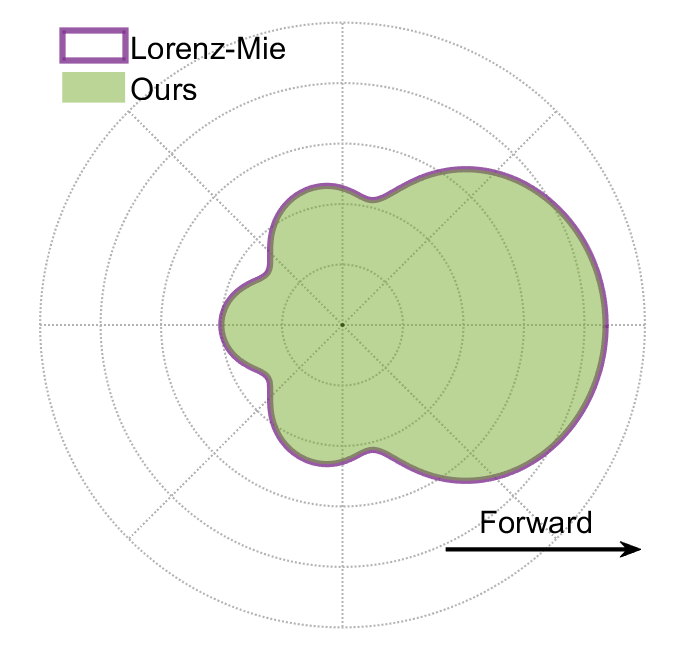
\includegraphics[width=\resLen]{images/pfunc/mie_300nm.png} & 
        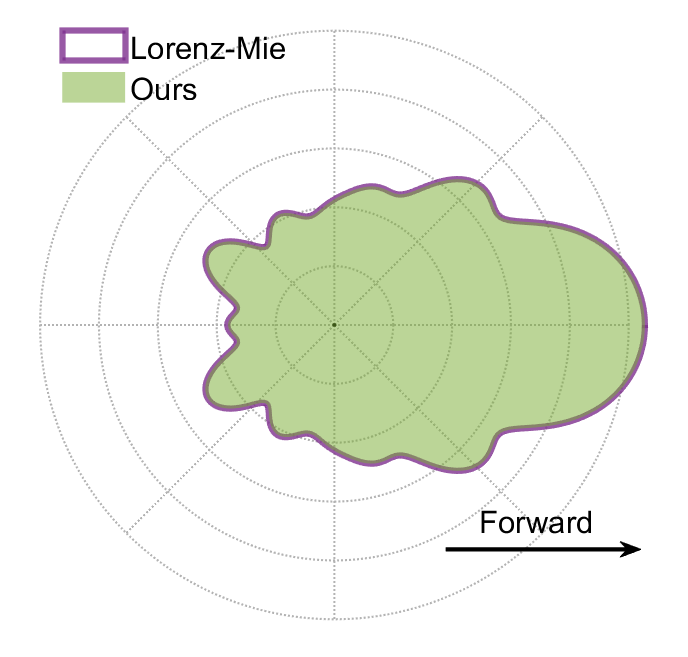
\includegraphics[width=\resLen]{images/pfunc/mie_600nm.png} &  
        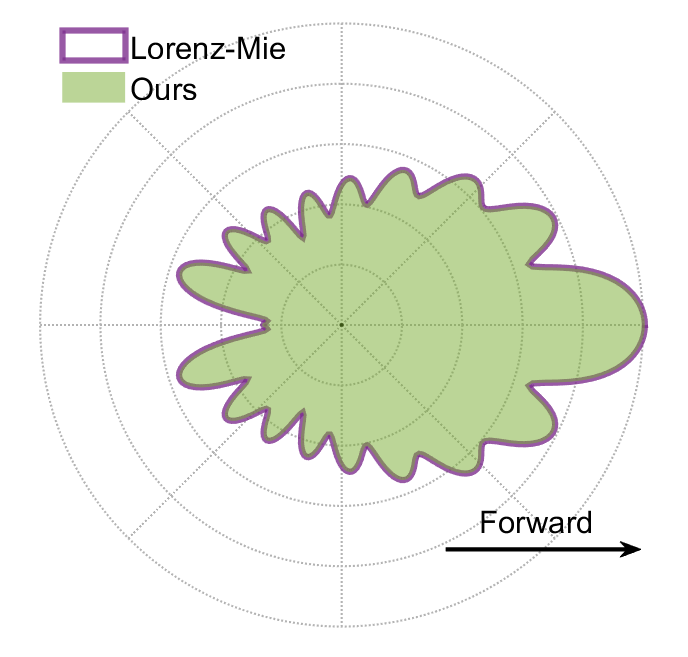
\includegraphics[width=\resLen]{images/pfunc/mie_900nm.png}  
        \\
        300nm & 600nm & 900nm
    \end{tabular}
    \caption{\label{fig:mie}
    Comparison against Lorenz-Mie theory: We compare our method with clusters containing a single particle (i.e., $\Ncls=1$) against a reference solution based on Lorenz-Mie theory for three different particle radii~$\radius_i \in \{ \text{300nm, 600nm, 900nm} \}$. As expected, for a single particle our method reduces to the same results as Lorenz-Mie theory. The wavelength is $\lambda=600$nm, while the refractive index of the particle is $\sIOR=1.5+0.1\img$.  
}
\end{figure}


\subsection{Relationship with the Radiative Transfer Theory}
\label{ssec:ours_RTT}
%
The scattering dyad $\ScaDyad_\Cls(\dwi,\dws)$ given by \Eq{eq:farscatdyadC} models how a particle cluster $\Cls$ scatters a planar unit-amplitude incident field in the far field region. However, for rendering we are generally interested on the average field intensity (i.e. radiance). 

As shown by Mishchenko~\shortcite{mishchenko2002vector}, the radiative transfer equation (RTE) directly derives from the far-field Foldy-Lax equations under three additional assumptions: (i)~The amount of coherent backscattering is negligible; (ii)~The particles are randomly distributed according to some distribution $p(\tPx_i,\Pprops_i)$, with $\tPx_i$ and $\Pprops_i$ denoting, respectively, the position and properties of a particle $i$; and (iii) We are interested on the average field $\EV{\EField(\px)}$. 

Following these assumptions, and after a lengthy derivation, Mishchenko demonstrates that the bulk scattering properties can be obtained from the far-field Foldy-Lax form, and in particular from the scattering dyad $\ScaDyad(\dwi,\dws)$. Let us first assume that the distribution of particle properties $\Pprops_i$ are independent of the particles position, and compute the average scattering dyad $\EV{\ScaDyad(\dwi,\dws)} = \int_\Omega \ScaDyad_i(\dwi,\dws) p(\Pprops_i) \diff{\Pprops_i}$. 
%
Then, note that the Foldy-Lax equation for clusters of particles~\eqref{eq:foldylaxcluster}, we derived above has the same form as the original Foldy-Lax equation~\eqref{eq:foldylax}. Thus, by the same derivation followed by Mishchenko we get to an equivalent RTE based on the scattering dyad of clusters. 

\paragraph{Computing the scattering parameters}
By taking the vectors of the parallel and perpendicular polarization $\dir{\boldsymbol\theta}^\text{inc}$ and $\dir{\boldsymbol\phi}^\text{inc}$ of the incident field as shown in Figure~\ref{fig:diagram} (right), and equivalently for the scattered field $\dir{\boldsymbol\theta}^\text{sca}$ and $\dir{\boldsymbol\phi}^\text{sca}$, we can compute the polarized scattering components $\ScaMatrix_\theta$ and $\ScaMatrix_\phi$ from the cluster's scattering dyad $\ScaDyad_\Cls(\dwi,\dws)$ as
%
\begin{align}
  \ScaMatrix_\theta(\dwi,\dws) &= \dir{\boldsymbol\theta}^\text{sca} \cdot \EV{\ScaDyad_\Cls(\dwi,\dws)} \cdot \dir{\boldsymbol\theta}^\text{inc}, \nonumber \\
  \ScaMatrix_\phi(\dwi,\dws) &= \dir{\boldsymbol\phi}^\text{sca} \cdot \EV{\ScaDyad_\Cls(\dwi,\dws)} \cdot \dir{\boldsymbol\phi}^\text{inc}.
\end{align}
%
Then, based on the two scattering components $\ScaMatrix_\theta$ and $\ScaMatrix_\phi$, we can obtain the optical parameters of the medium as
%
\begin{align}
    \label{eq:crosstcluster}
    \cT(\dwi) &= 4\pi \Re\left[\frac{\ScaMatrix(\dwi,\dwi)}{k_i^2}\right], \\
    \label{eq:crossscluster}
    \cS(\dwi) &=\int_\Sph \frac{|\ScaMatrix_\theta(\dwi,\dws)|^2+|\ScaMatrix_\phi(\dwi,\dws)|^2}{2k_1^2} \diff{\dws}, \\
    \label{eq:phasecluster}
    \phase(\dwi,\dws) &= \frac{|\ScaMatrix_\theta(\dwi,\dws)|^2+|\ScaMatrix_\phi(\dwi,\dws)|^2}{2k_1^2\cS},
\end{align}
%
with $\ScaMatrix(\dwi,\dwi)=\ScaMatrix_\phi(\dwi,\dwi)=\ScaMatrix_\theta(\dwi,\dwi)$, and $\Re[x]$ returning the real part of a complex number $x$. Lastly, assuming a uniform distribution of clusters, we can compute the extinction and scattering coefficients as
%
\begin{align}
    \label{eq:sigmatcluster}
    \sigT(\dwi) &= \cT(\dwi) \frac{\rho}{\EV{\Ncls}}, \\
    \label{eq:sigmascluster}
    \sigS(\dwi) &= \cS(\dwi) \frac{\rho}{\EV{\Ncls}},
\end{align}
%
with $\rho$ the number of particles per differential volume, and $\EV{\Ncls}$ the average number of particles per cluster. Note that the optical properties defined in Equations~\eqref{eq:crosstcluster}--\eqref{eq:sigmascluster} are directionally dependent, so they are general and can represent both isotropic and anisotropic media. 

\begin{figure}
    \centering
    \setlength{\resLen}{3.5in}
    \addtolength{\tabcolsep}{-3pt}
    \begin{tabular}{c}
        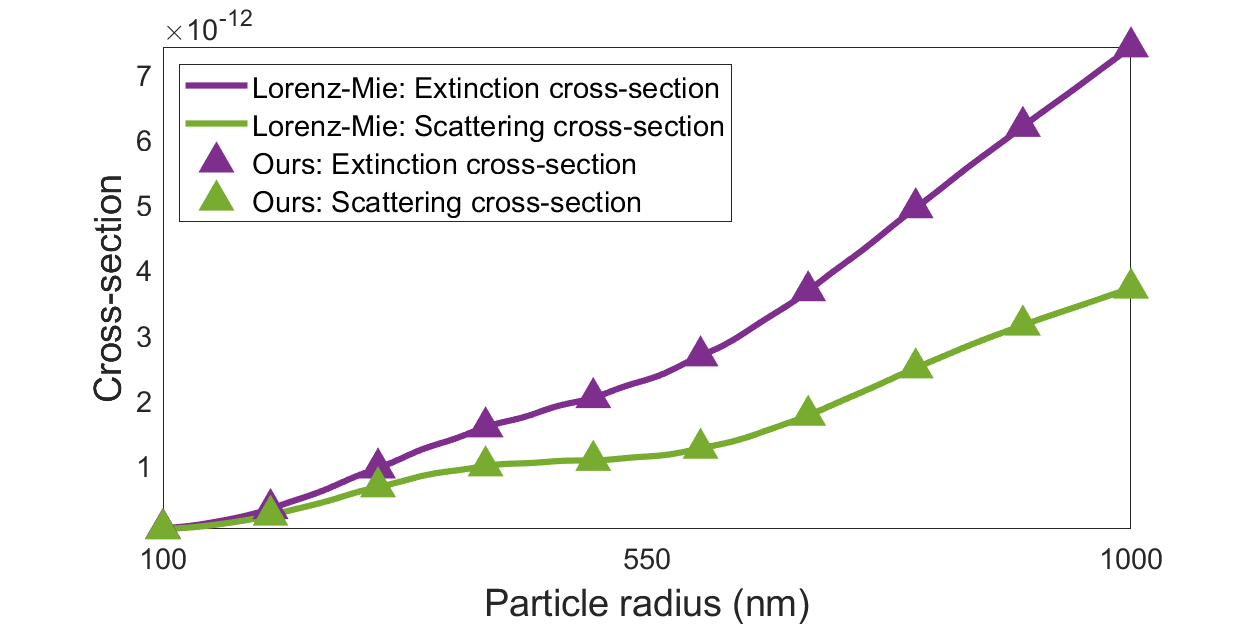
\includegraphics[width=\resLen]{images/pfunc/CsCt.png} 
    \end{tabular}
    \caption{
        Comparison against Lorenz-Mie theory: We compare the extinction and scattering cross sections computed with our method for $\Ncls=1$ against the results obtained using Lorenz-Mie theory. As in Figure~\ref{fig:mie} our results show perfect agreement. 
    \label{fig:mie2}
}
\end{figure}

\begin{figure*}[t]
    \centering
    \setlength{\resLenTwo}{2in}
    \setlength{\resLen}{.1\textwidth}
    \addtolength{\tabcolsep}{-3pt}
    \small
    \begin{tabular}{ccc|ccc|ccc}
        \multicolumn{3}{c|}{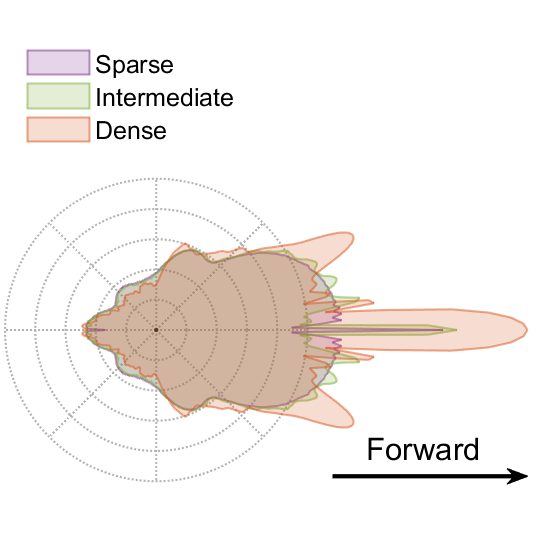
\includegraphics[height=\resLenTwo]{images/pfunc/distance.png}} &
        \multicolumn{3}{c|}{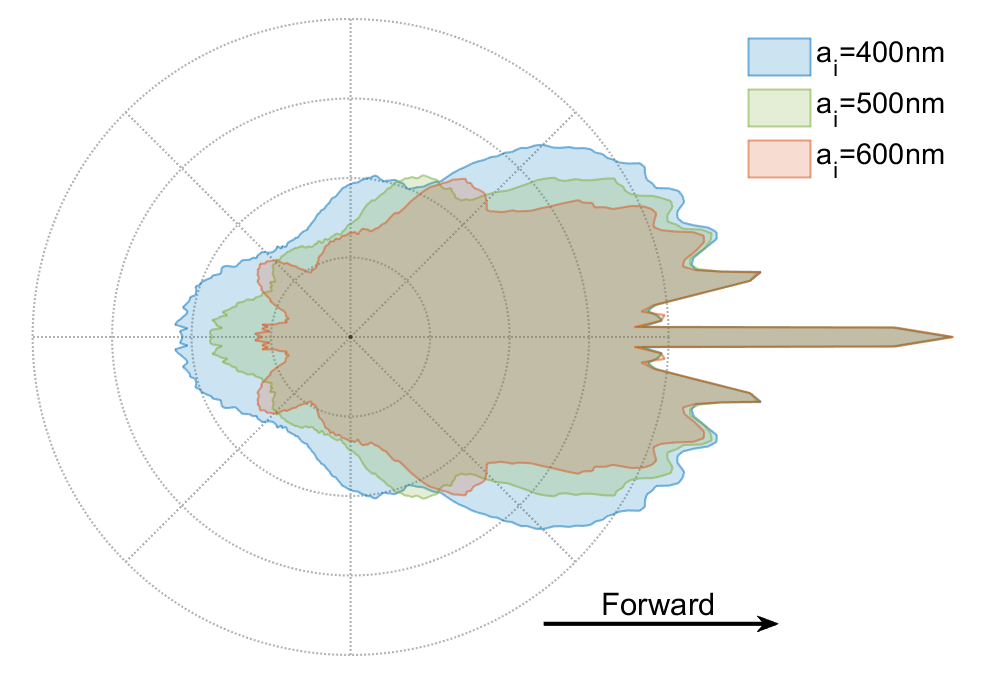
\includegraphics[height=\resLenTwo]{images/pfunc/radius.png}} &
        \multicolumn{3}{c}{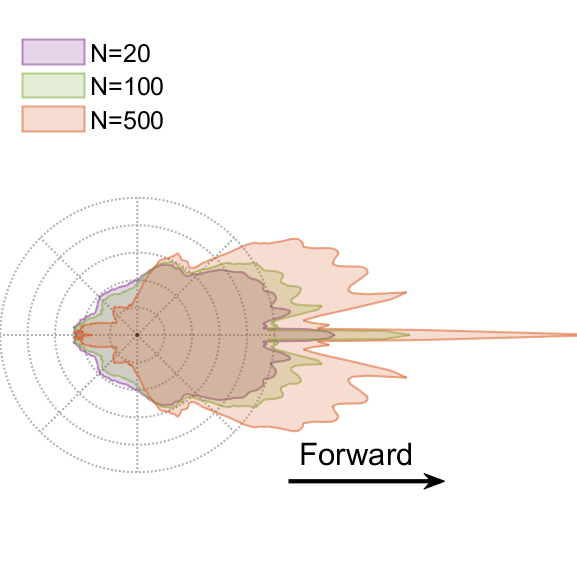
\includegraphics[height=\resLenTwo]{images/pfunc/number.png}} \\[-5pt]
        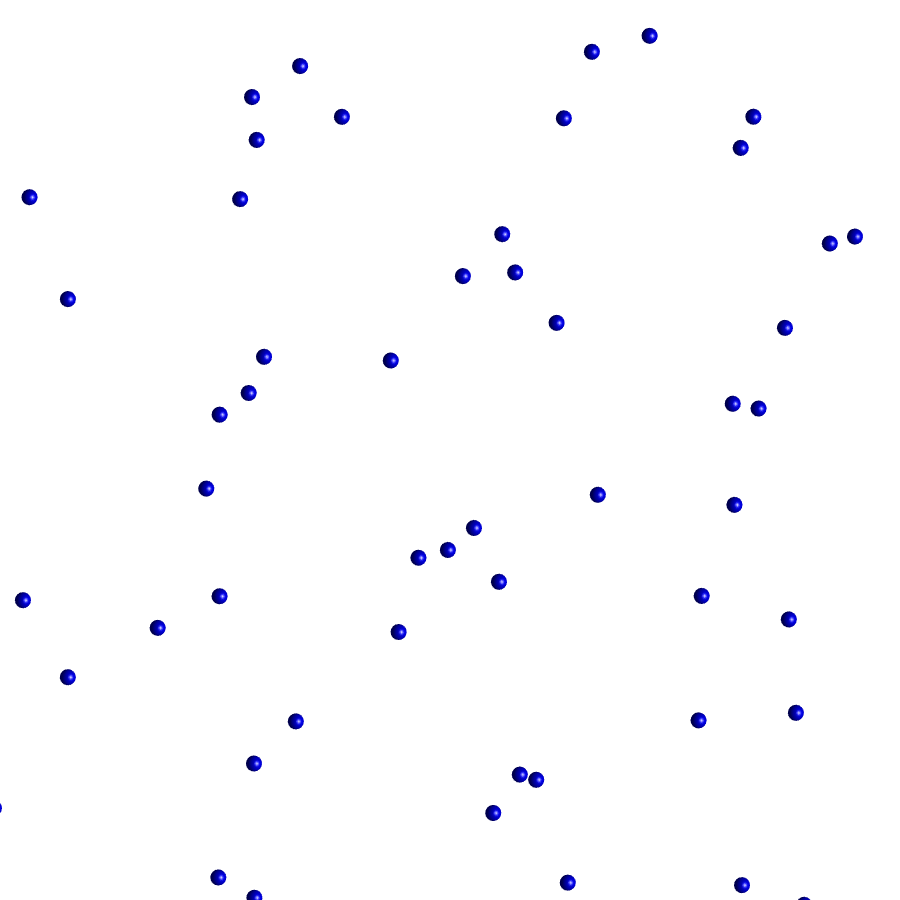
\includegraphics[width=\resLen]{images/particle/validate2_D1_N100_500nm.png} &
        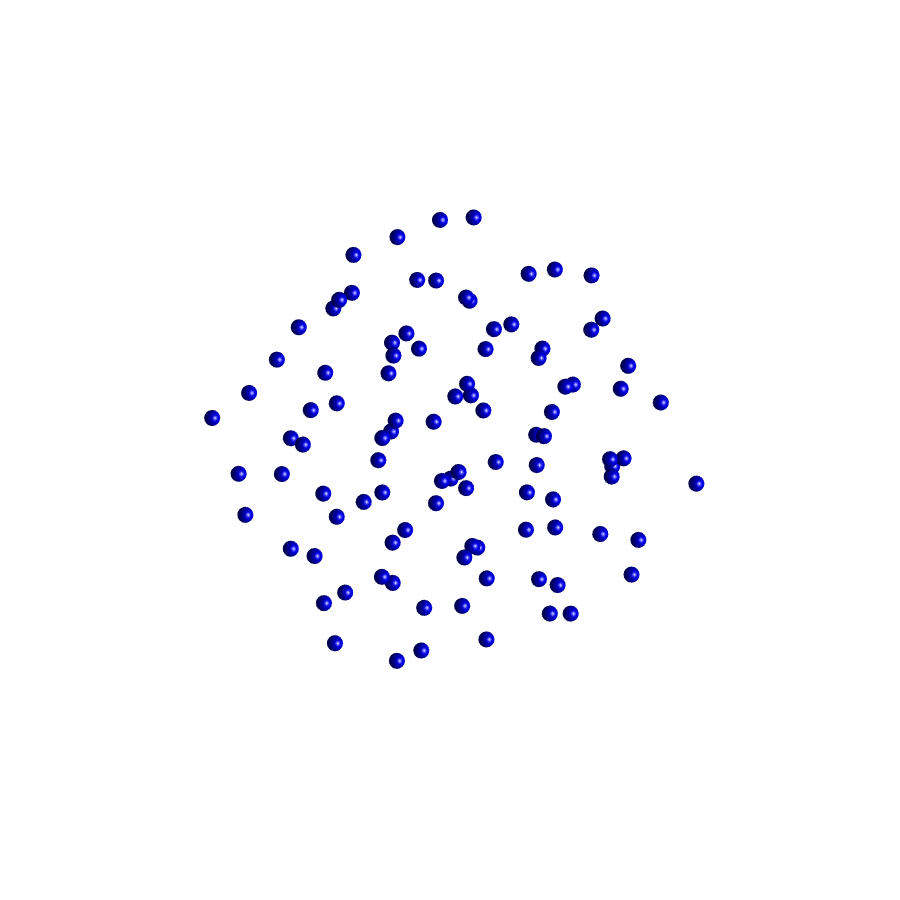
\includegraphics[width=\resLen]{images/particle/validate3_D2_N100_500nm.png} &
        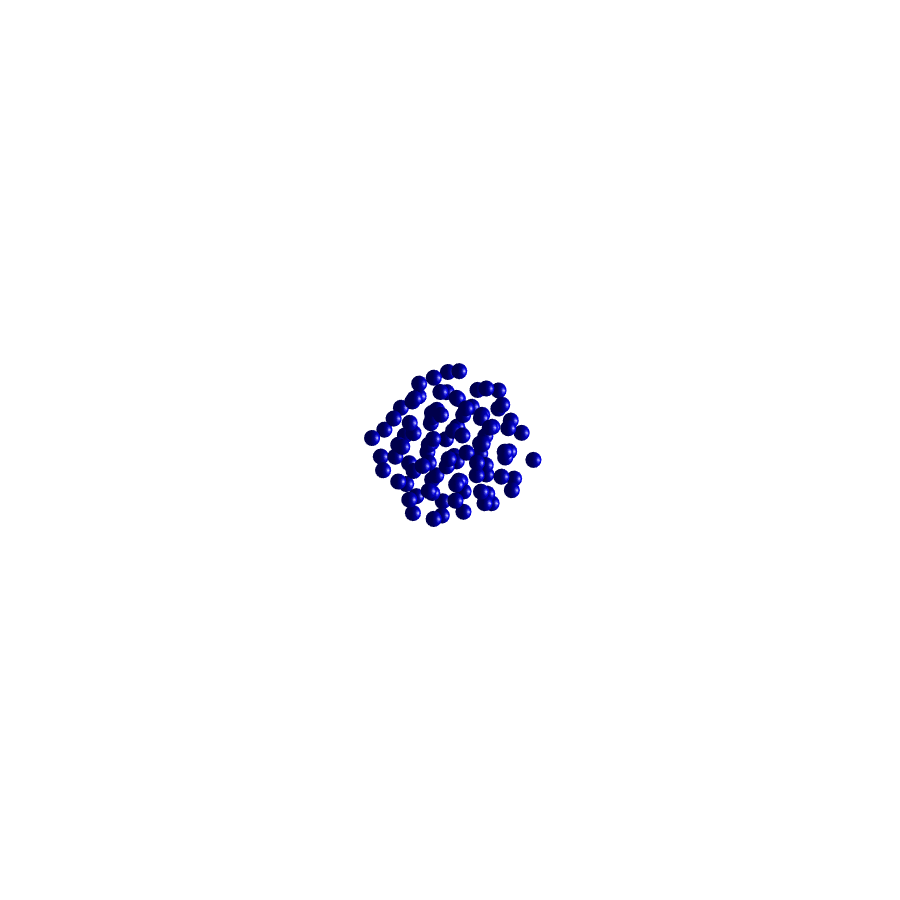
\includegraphics[width=\resLen]{images/particle/validate4_D3_N100_500nm.png} &
        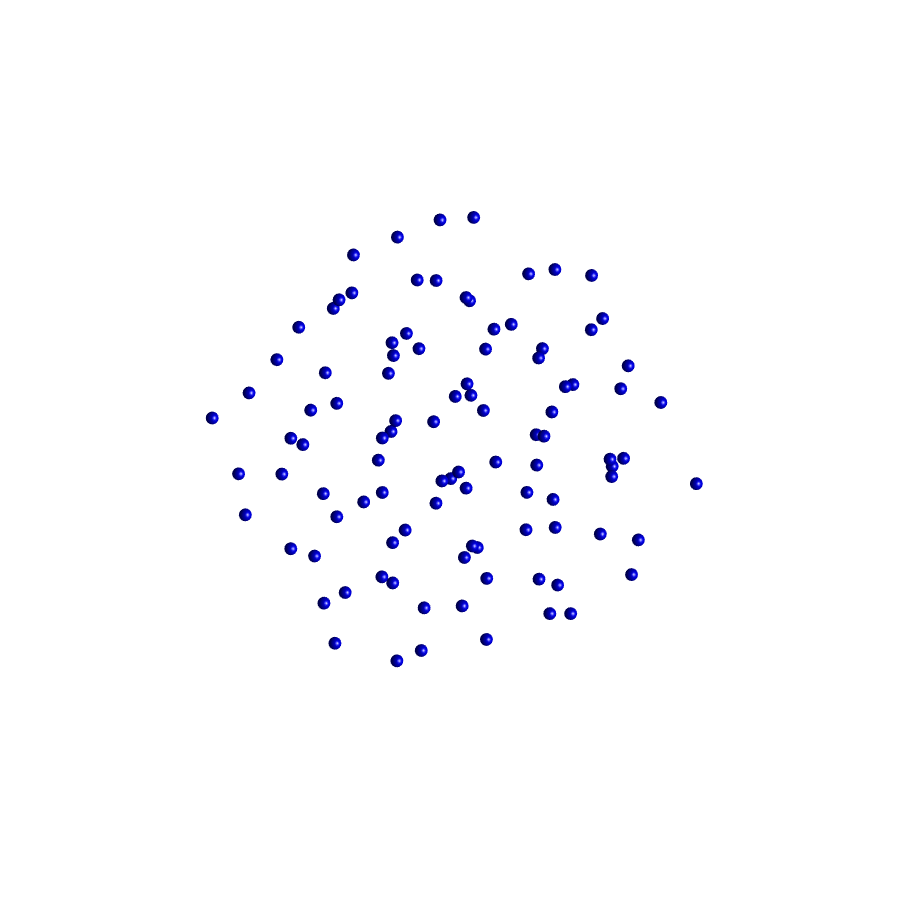
\includegraphics[width=\resLen]{images/particle/validate5_D2_N100_400nm.png} &
        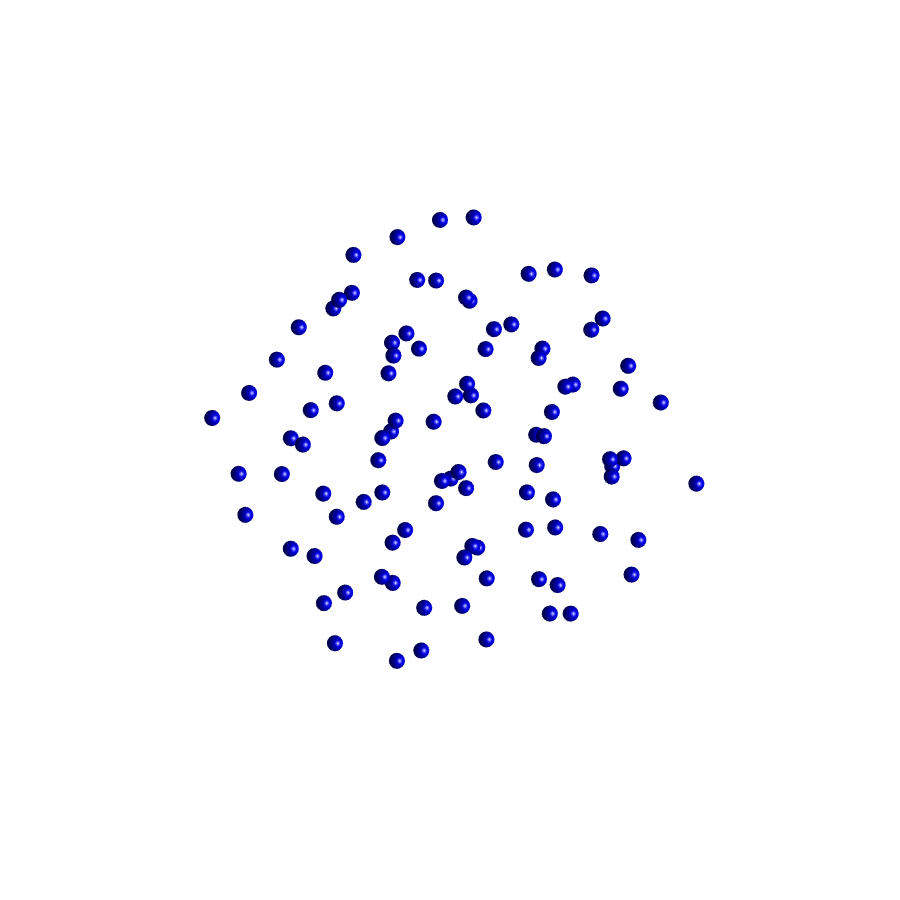
\includegraphics[width=\resLen]{images/particle/validate3_D2_N100_500nm.png} &
        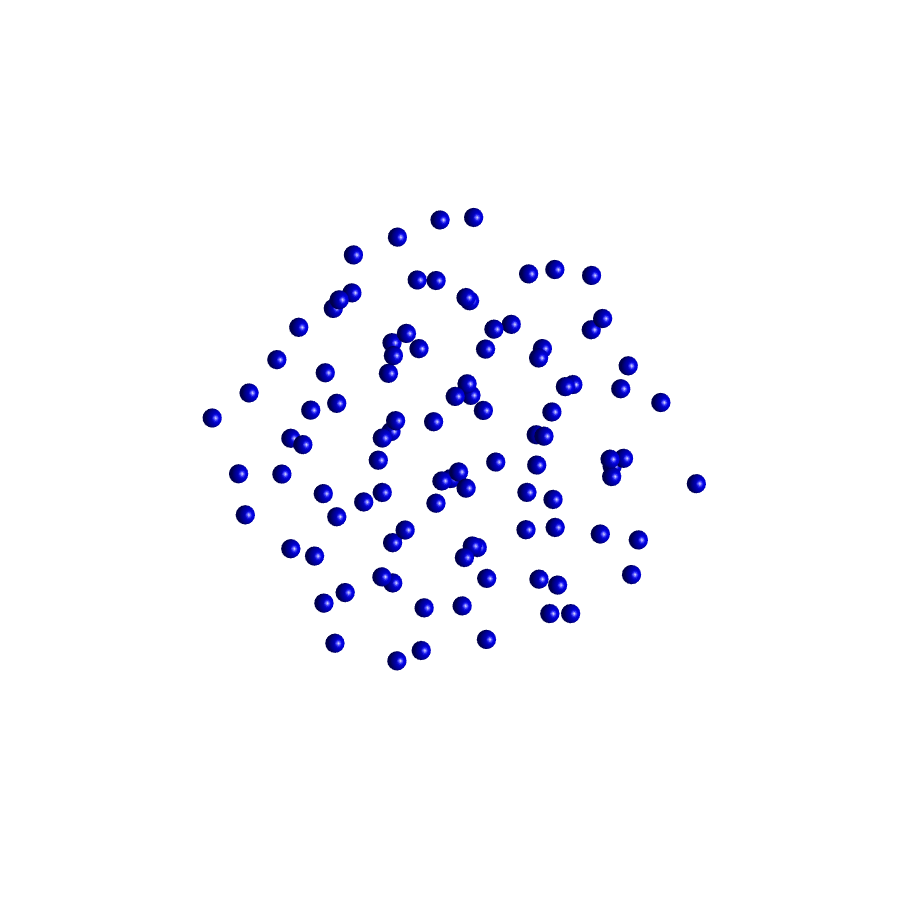
\includegraphics[width=\resLen]{images/particle/validate7_D2_N100_600nm.png} &
        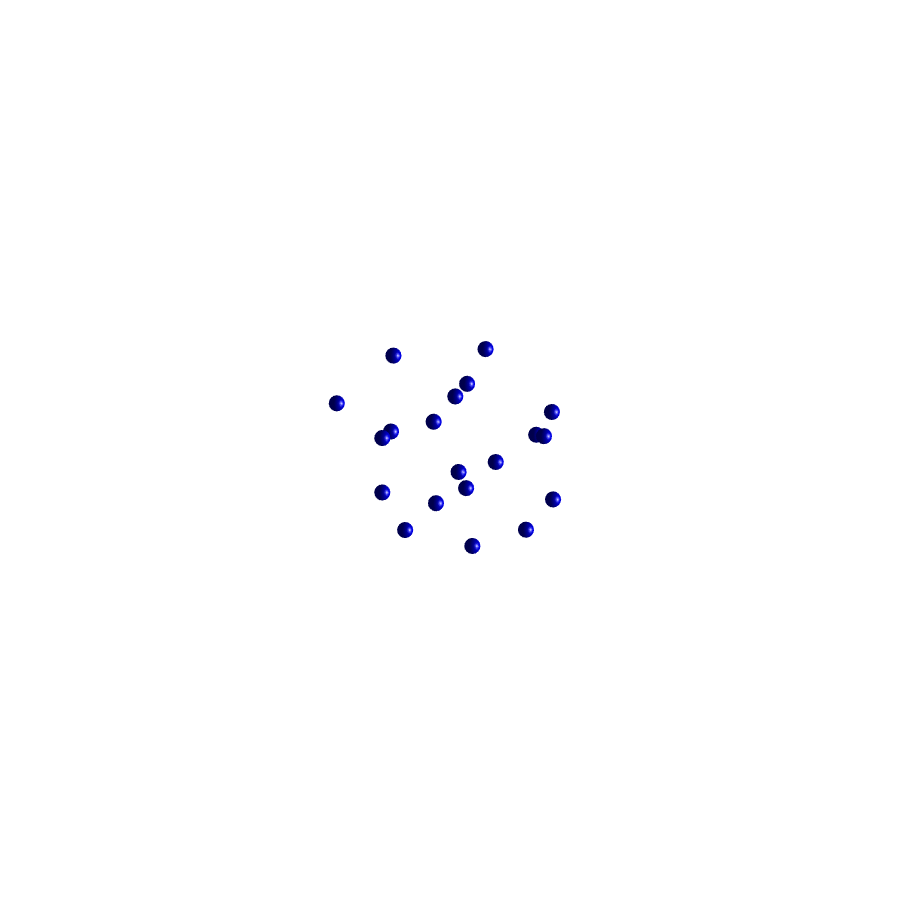
\includegraphics[width=\resLen]{images/particle/validate8_D2_N20_500nm.png} &
        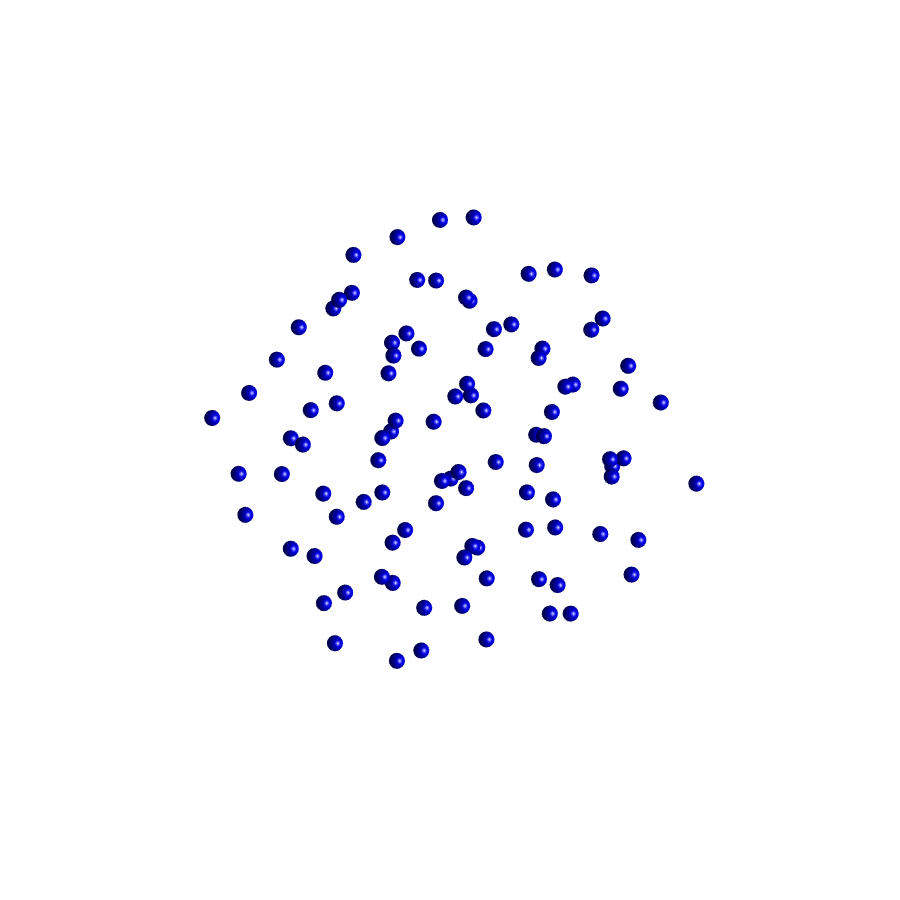
\includegraphics[width=\resLen]{images/particle/validate3_D2_N100_500nm.png} &
        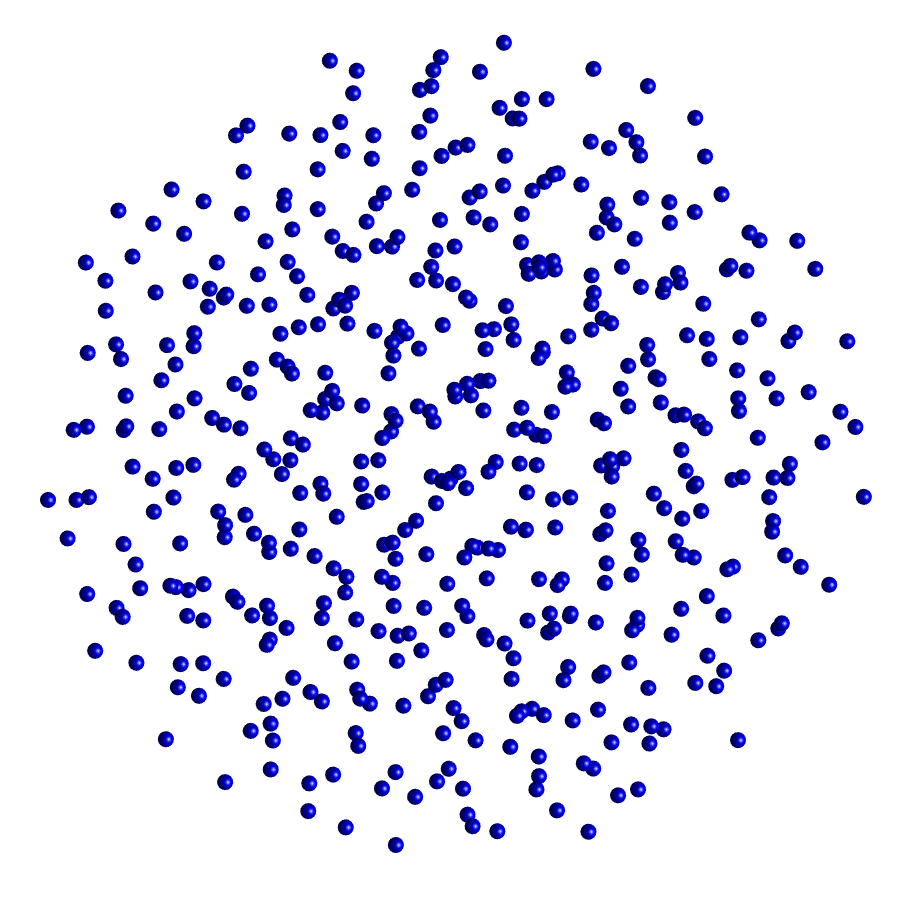
\includegraphics[width=\resLen]{images/particle/validate10_D2_N500_500nm.png} 
        \\
        Sparse & Intermediate & Dense & $\radius_i$=400nm & $\radius_i$=500nm & $\radius_i$=600nm &
        $\Ncls=20$ & $\Ncls=100$ & $\Ncls=500$ \\[5pt]
        \multicolumn{3}{c}{\bfseries (a) Varying particles spacing} &
        \multicolumn{3}{c}{\bfseries (b) Varying particles radius} &
        \multicolumn{3}{c}{\bfseries (c) Varying particles count}
    \end{tabular}
    \caption{\label{fig:ablation}
        Comparison of the resulting phase function for different cluster parameters, for a planar incident field at $\lambda=700$nm. Unless mentioned otherwise, the clusters have $\Ncls=100$ particles, and each particle has radius $\radius_i=500$nm. For each phase function, we vary: (a) The distance between particles within the cluster; (b) The particle size $\radius_i$; and (c) The number of particles $\Ncls$. 
    }
\end{figure*}

\subsection{Relationship with Independent Scattering}
\label{ssec:ours_indep_scat}
%
Most previous works rendering light transport in media~\cite{novak2018monte} build on the assumption of independent scattering---that is, particles are in their respective far-field region.
It is easy to verify that this is a special case of \Eq{eq:foldylaxtwo} with $\Ncls=1$, causing 
the scattering dyad $\ScaDyad_\Cls$ of \Eq{eq:farscatdyadC} to reduce to
%
\begin{equation}
    \label{eq:farscatmie}
    \ScaDyad_\Cls(\dwi,\dws) = \ScaDyad_i(\dwi,\dws) = \frac{g(\dws)\cdot \dyad{T}_i  \cdot\sGreenProp(\dwi)}{4\pi},
\end{equation}
%
which encodes the scattered field in the far-field region of a particle when excited by an incident unit-amplitude planar field. 
%
The Lorenz-Mie theory~\cite{hulst1981light} provides closed-form expressions for $\ScaDyad_i(\dwi,\dws)$ for spheres and cylinders, while numerical solutions of $\ScaDyad_i(\dwi,\dws)$ have been proposed for scatterers of arbitrary shapes via, for example, the T-matrix method~\cite{waterman1965matrix}, or more recently based on the BEM for cylindrical fibers~\cite{xia2020wave}. Our work is therefore a generalization of these works to particles in the near field. 
